\documentclass[a4paper,14pt]{extarticle}

\usepackage[utf8x]{inputenc}
\usepackage[T1]{fontenc}
\usepackage[russian]{babel}
\usepackage{hyperref}
\usepackage{indentfirst}
\usepackage{here}
\usepackage{array}
\usepackage{graphicx}
\usepackage{grffile}
\usepackage{caption}
\usepackage{subcaption}
\usepackage{chngcntr}
\usepackage{amsmath}
\usepackage{amssymb}
\usepackage{pgfplots}
\usepackage{pgfplotstable}
\usepackage[left=2cm,right=2cm,top=2cm,bottom=2cm,bindingoffset=0cm]{geometry}
\usepackage{multicol}
\usepackage{multirow}
\usepackage{titlesec}
\usepackage{listings}
\usepackage{color}
\usepackage{longtable}
\usepackage{enumitem}
\usepackage{cmap}
\usepackage{tikz}

\usetikzlibrary{shapes,arrows}

\definecolor{green}{rgb}{0,0.6,0}
\definecolor{gray}{rgb}{0.5,0.5,0.5}
\definecolor{purple}{rgb}{0.58,0,0.82}

\lstset{
	language={SQL},
	inputpath={../},
	backgroundcolor=\color{white},
	commentstyle=\color{green},
	keywordstyle=\color{blue},
	numberstyle=\scriptsize\color{gray},
	stringstyle=\color{purple},
	basicstyle=\small,
	breakatwhitespace=false,
	breaklines=true,
	captionpos=b,
	keepspaces=true,
	numbers=left,
	numbersep=5pt,
	showspaces=false,
	showstringspaces=false,
	showtabs=false,
	tabsize=8,
	frame=single,
}

\renewcommand{\le}{\ensuremath{\leqslant}}
\renewcommand{\leq}{\ensuremath{\leqslant}}
\renewcommand{\ge}{\ensuremath{\geqslant}}
\renewcommand{\geq}{\ensuremath{\geqslant}}
\renewcommand{\epsilon}{\ensuremath{\varepsilon}}
\renewcommand{\phi}{\ensuremath{\varphi}}
\renewcommand{\thefigure}{\arabic{figure}}
\def\code#1{\texttt{#1}}

\titleformat*{\section}{\large\bfseries} 
\titleformat*{\subsection}{\normalsize\bfseries} 
\titleformat*{\subsubsection}{\normalsize\bfseries} 
\titleformat*{\paragraph}{\normalsize\bfseries} 
\titleformat*{\subparagraph}{\normalsize\bfseries} 

\counterwithin{figure}{section}
\counterwithin{equation}{section}
\counterwithin{table}{section}
\newcommand{\sign}[1][5cm]{\makebox[#1]{\hrulefill}}
\newcommand{\equipollence}{\quad\Leftrightarrow\quad}
\newcommand{\no}[1]{\overline{#1}}
\graphicspath{{../}}
\captionsetup{justification=centering,margin=1cm}
\def\arraystretch{1.3}
\setlength\parindent{5ex}
\titlelabel{\thetitle.\quad}

\setitemize{itemsep=0em}
\setenumerate{itemsep=0em}

\tikzstyle{startstop} = [
	rectangle,
	align=center,
	rounded corners,
	text width=10em,
	text centered,
	draw=black
]
\tikzstyle{process} = [
	rectangle,
	align=center,
	text width=20em,
	text centered,
	draw=black
]
\tikzstyle{decision} = [
	diamond,
	aspect=4,
	align=center,
	inner sep=0pt,
	text width=10em,
	text centered,
	node distance=5em,
	draw=black
]
\tikzstyle{line} = [
	draw=black,
	thick,
	->,
	>=stealth,
	-latex'
]

\begin{document}

\begin{titlepage}
\begin{center}
	САНКТ-ПЕТЕРБУРГСКИЙ ПОЛИТЕХНИЧЕСКИЙ УНИВЕРСИТЕТ\\ ПЕТРА ВЕЛИКОГО\\[0.3cm]
	\par\noindent\rule{10cm}{0.4pt}\\[0.3cm]
	Институт компьютерных наук и технологий \\[0.3cm]
	Кафедра компьютерных систем и программных технологий\\[4cm]
	
	Отчет по лабораторной работе № 1\\[3mm]
	Дисциплина: <<Базы данных>>\\[3mm]
	Тема: <<Разработка структуры БД>>\\[7cm]
\end{center}

\begin{flushleft}
	\hspace*{5mm} Выполнил студент гр. 43501/3  \hspace*{2.5cm}\sign[3cm]\hspace*{3.0mm} А.Ю. Ламтев\\
	\hspace*{10.4cm} (подпись)\\[3mm]
	\hspace*{5mm} Преподаватель \hspace*{6.0cm}\sign[3cm]\hspace*{2mm} А.В. Мяснов\\
	\hspace*{10.4cm} (подпись)\\[3mm]
	\hspace*{11.1cm} <<\sign[7mm]>> \sign[27mm] \the\year\hspace{1mm} г.
\end{flushleft}

\vfill

\begin{center}
	Санкт-Петербург\\
	\the\year
\end{center}
\end{titlepage}
\addtocounter{page}{1}

\tableofcontents
\newpage

\section{Цели работы}

Познакомиться с основами проектирования схемы БД, языком описания сущностей и ограничений БД SQL-DDL.

\section{Программа работы}

\begin{enumerate}
	\item Самостоятельное изучение SQL-DDL.
	\item Создание скрипта БД в соответствии с согласованной схемой. Должны присутствовать первичные и внешние ключи, ограничения на диапазоны значений. Демонстрация скрипта преподавателю. 
	\item Создание скрипта, заполняющего все таблицы БД данными.
	\item Выполнение SQL-запросов, изменяющих схему созданной БД по заданию преподавателя. Демонстрация их работы преподавателю.
\end{enumerate}
 
\section{Создание скрипта БД в соответствии с согласованной схемой} 
 
На рис. \ref{fig:movie-service-diagram-old} изображена согласованная схема БД.

\begin{figure}[H]
	\centering
	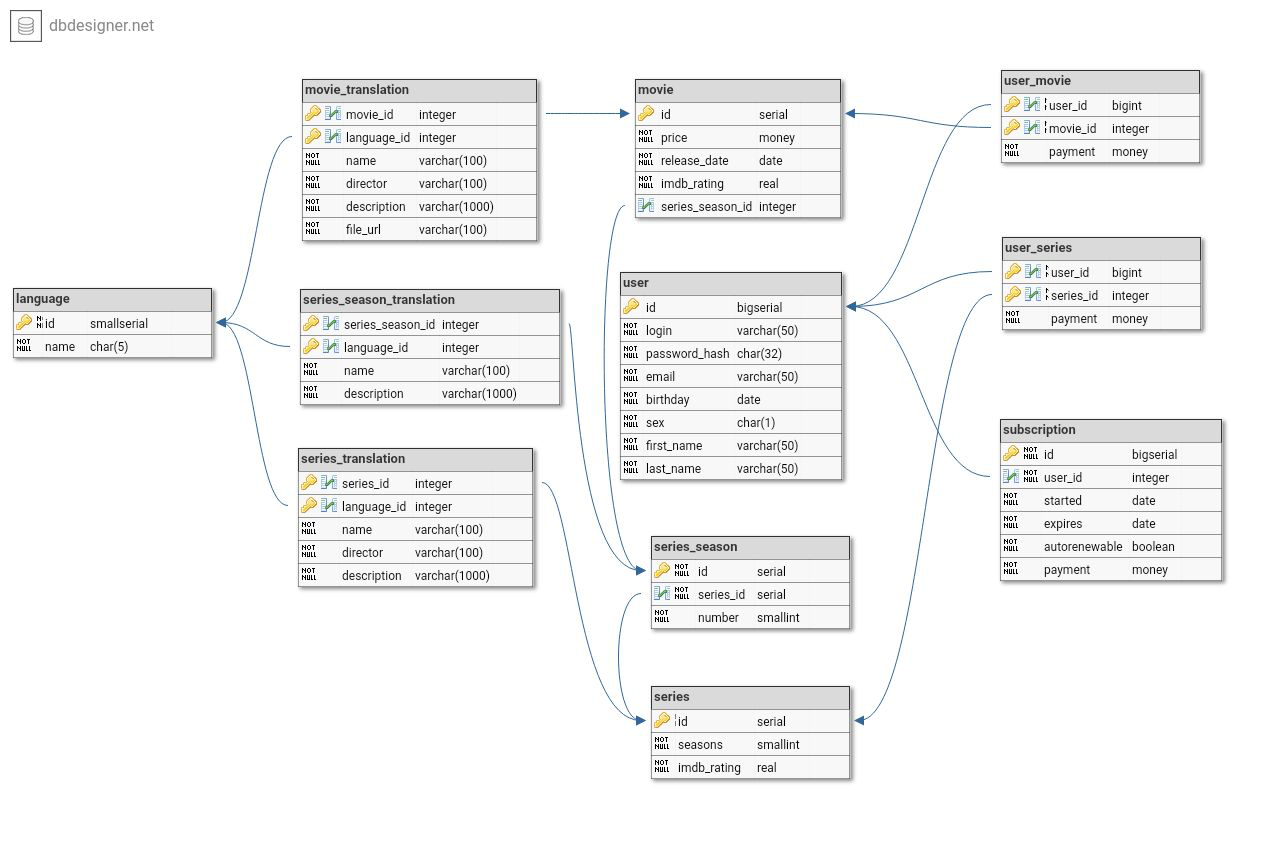
\includegraphics[width=1.0\textwidth]{../../lab1/diagrams/movie-service-diagram}
	\caption{Согласованная схема БД}
	\label{fig:movie-service-diagram-old}
\end{figure}

В листинге \ref{lst:create} представлен скрипт, создающий БД в соответствии с согласованной схемой, изображённой на рис. \ref{fig:movie-service-diagram}.

\lstinputlisting[caption={Скрипт, создающий БД в соответствии с согласованной схемой},label={lst:create}]{sql/create.sql}

Затем заполним созданную базу данными. Скрипт заполнения приведён в листинге \ref{lst:insert}.

\lstinputlisting[caption={Скрипт, заполняющий базу данными},label={lst:insert}]{sql/insert.sql}

\section{Изменение схемы БД}

Заданием было внести изменения в схему БД для удовлетворения следующим требованиям:

\begin{enumerate}
	\item  Ввести возможность подписок на часть фильмов/сериалов.
	\item  Реализовать каталог фильмов и сериалов по различным категориям: жанры, новинки и пр. Каждый фильм может быть отнесен к нескольким категориям. Категории могут иметь иерархию, но при этом фильмы могут относиться к узлу любого уровня иерархии.
\end{enumerate}

В соответствии с заданием схема БД была изменена, и она приняла следующий вид:

\begin{figure}[H]
	\centering
	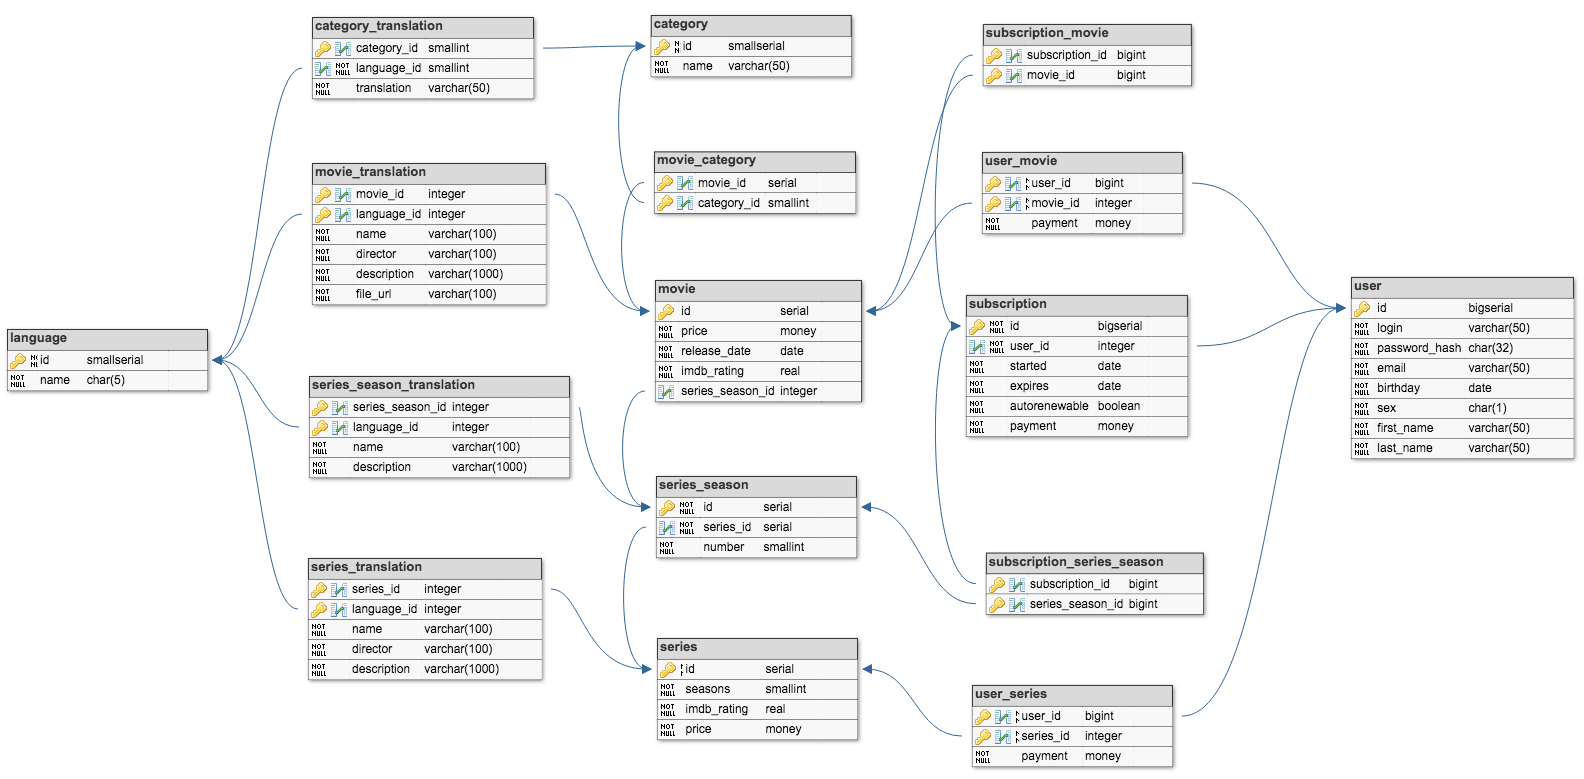
\includegraphics[width=1.0\textwidth]{diagrams/movie-service-diagram}
	\caption{Изменённая схема БД}
	\label{fig:movie-service-diagram}
\end{figure}

В сравнении с предыдущей версией были добавлены следующие таблицы: \code{subscription\_movie}, \code{subscription\_series\_season}, \code{category}, \code{movie\_category} и \code{category\_translation}.

В листинге \ref{lst:update} представлен скрипт, вносящий изменения в БД в соответствии с новой схемой, изображённой на рис. \ref{fig:movie-service-diagram}, а также заполняющий базу новыми данными.

\lstinputlisting[caption={Скрипт, вносящий изменения в БД},label={lst:update}]{sql/update.sql}

\section{Выводы}

В результате работы было проведено ознакомление с языком SQL-DDL, был разработан скрипт, создающий базу данных в соответствии с выбранной ранее моделью данных. Затем было осуществлено изменение модели данных и был разработан скрипт, обновляющий базу данных в соответствии с новой схемой.

\end{document}
